\chapter{Case study} \label{sec:4}


This chapter will explain the experiment used in the Study Case.   Three versions of EvoDrawing were used to fulfill this research.

Starting off with the hypothesis which will allow increasing the user experience of having a drawing modeling using diffuse logic and use techniques.

It was necessary to design Three experiments to prove this thesis work hypothesis; each experiment used a different version of EvoDrawing.  The results as well as each version of EvoDrawing compared to other applications of interactive evolutionary computing and also were compared between other Evo Drawing versions itself.  Equality of data, parameters, and users compared to all experiments which examined as follows:

It is necessary to compare our proposal with other which we have explained early in the last chapter, due evolutionary interactive computing applications with the same amount of parameters are difficult to find we decided to build two additional ones in order to run pertinent tests so our hypothesis could be answered., This required to design experiments the following way.

The X table contains Evo Drawing versions and comparison. The first column will specify each version of Evo Drawing including its characteristics and each subsequent column describes the characteristics of each Evo Drawing version.

\begin{table}
	\small
	\caption{comparison of the different versions.}
	\label{tab:comparison} 
	\centering
	\small
	\begin{tabular}{p{3cm} p{4cm} p{4cm} p{4cm} }
		\hline\noalign{\smallskip}
		Version & EvoDrawing01 & EvoDrawing02 & EvoDrawing03 \\
		\noalign{\smallskip}\hline\noalign{\smallskip}
		\small{User Interface} & \small{This version have an easy to handle and simple gui.Observe figure X} & \small{This version have an easy to handle and simple gui. Observe figure X} & \small{As the previous versions this one have the same interface but differs from the others on the competitiveness visual components based on video games and we can observe it in figure X}\\ \hline
		\small{Fuzzy Inferance} & \small{It does not have Fuzzy inference system} & \small{A fuzzy inference system has been added to this version.  It is composed by two inputs Experience and Preference; it also has a type Mamdani output called fuzzy rate.} & \small{A fuzzy inference system has been added to this version.  It is composed by three inputs Ranking, Experience and Preference; it also has a type Mamdani output called fuzzy rate.
			}\\ \hline 
		\small{Graph-based user model} & \small{User modeling is not available} & \small{User modeling is not available} & \small{User modeling is available in this version based on graphs and is used to adapt inside diffuse inference aptitude function on ranking entrance.
		}\\ \hline 
		
		\noalign{\smallskip}\hline
	\end{tabular}
\end{table}

Now we will explain each version developed details and goes as follows; we will explain each version specific and technical reasons.





\section{EvoDrawings01} 


This version initial configuration of our evolutionary algorithm goes as follows:

\begin{enumerate}
	\item  \textbf{Having an initial 80 individual population which we will represent in the following way:}
	
	
	
	\item  \textbf{evaluations equals an evolution parameter.}
	 
	\item  \textbf{Its fitness provided by equation x.} 
	\item  \textbf{Combining the fuzzified inputs according to the fuzzy rules to establish a rule strength.} 
	\item  \textbf{Combining the consequences to get an output distribution.}
	\item  \textbf{Defuzzifying the  output distribution (this step is only if a crisp production (class) is needed).}
\end{enumerate}











\subsection{Interface.} 

An easy use individual evaluation web interface is develop to this version.  We can notice in the navigation bar the access application functionality, worth mentioning that the app will only work with the social platform Facebook. Once accessed with a Facebook account the navigation bar will show an avatar as well as the exit application functionality through a logout. Also inside this interface exist the visual element “Friends” that will show all the participating friends in the form, to be able to view friend’s public collections is another functionality this element has.
Continuing with the interface explanation, we found the “Collections” panel where the user's list of created and saved collections is shown as well as the functionality that give the ability to create new collections. An “About this” section will be shown inside; this will explain in a general way the functionality to the participating users. Now when it comes to user’s individual evaluation they will have a visual canvas element who will show behavior of a to be evaluated individual (animation) and in the lower part the individual will have the ability to star rank evaluate where one star means he/she did not like it much and five stars meaning he/she like it too much. Now in the lower section of the star rank, a button will provide the ability to add that individual to a collection previously created. In the upper-rank star section, we will find a link which reads “Click here to see my DNA History” this will take us to detail about the individual to be evaluated that way we could review the detail of the individual in image x.

\begin{figure*}
	%\captionsetup{justification=centering,margin=2cm}
	\centering
	\setlength\fboxsep{0pt}
	\fbox{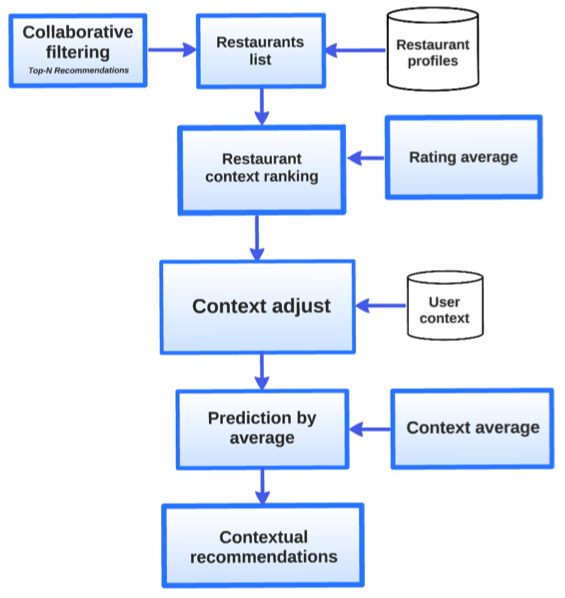
\includegraphics[width=0.60\textwidth]{img/posfil.png}}
	\caption{The Post-Filtering architecture for Tijuana restaurants.}
	\label{fig:postfiltering}     
\end{figure*}


Detailed Important information about individual DNA history is shown here such as how many evaluations in likes he/she has received, how many visitors as well as ascendancy, genetic crossing operator, chromosome numeric representation and inside population identifier.


\begin{figure*}
	%\captionsetup{justification=centering,margin=2cm}
	\centering
	\setlength\fboxsep{0pt}
	\fbox{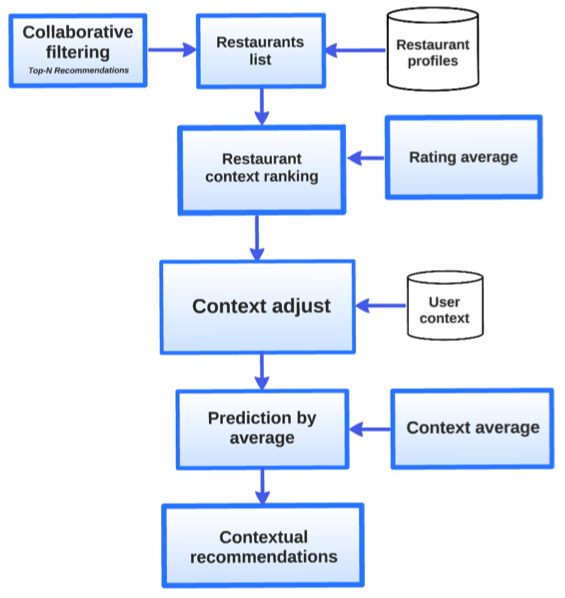
\includegraphics[width=0.60\textwidth]{img/posfil.png}}
	\caption{The Post-Filtering architecture for Tijuana restaurants.}
	\label{fig:postfiltering}     
\end{figure*}

\section{EvoDrawing02}

Inside this version we will find an initial configuration of the interactive evolutionary algorithm in the following way:

As in the Las version it counts with 80 individuals as initial population and individuals are represented in the same way as in the previous version:
Eight evaluations as one evolution parameter.
One genetic Operator as aleatory selection between competition and ...      
One horizontal genetic crossing Operator.
Its fitness function is provided by equation x.

\begin{enumerate}
	\item  \textbf{Having an initial 80 individual population which we will represent in the following way:}
	
	
	
	\item  \textbf{As in the Las version it counts with 80 individuals as initial population and individuals are represented in the same way as in the previous version.}
	
	\item  \textbf{Eight evaluations as one evolution parameter..} 
	\item  \textbf{Combining the fuzzified inputs according to the fuzzy rules to establish a rule strength.} 
	\item  \textbf{One genetic Operator as aleatory selection between competition and ...}
	\item  \textbf{Its fitness function is provided by equation x.}
\end{enumerate}

\begin{figure*}
	%\captionsetup{justification=centering,margin=2cm}
	\centering
	\setlength\fboxsep{0pt}
	\fbox{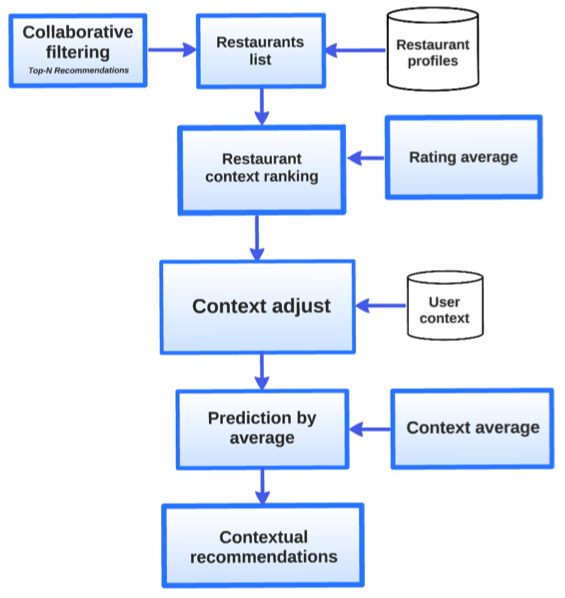
\includegraphics[width=0.60\textwidth]{img/posfil.png}}
	\caption{The Post-Filtering architecture for Tijuana restaurants.}
	\label{fig:postfiltering}     
\end{figure*}



\subsection{Fuzzy Inferance.}
Where represents all the individuals.
Is the rank given to the individuals by the users.
Represents one diffuse rank function composed by a diffuse inference system and will be represented by equation x.


Where represents the diffuse rank.
Will continue been users given rank according to their preferences to each.
Is the experience which is defined by the activity already explained in the previous chapter.

The diffuse inference system type is Mamdani, and it is composed by two entrances represented by and a fuzzy rate exit as we can observe represented in figure x.


It counts with 9 if/then rules which were designed in an empiric way and are the following:

If experience is low and preference is low then fuzzy\_rate is bad
If experience is mid and preference is low then fuzzy\_rate is bad
If experience is high and preference is low then fuzzy\_rate is normal
If experience is low and preference is mid then fuzzy\_rate is bad
If experience is mid and preference is mid then fuzzy\_rate is normal
If experience is high and preference is mid then fuzzy\_rate is good
If experience is low and preference is high then fuzzy\_rate is normal
If experience is mid and preference is high then fuzzy\_rate is good
If experience is high and preference is high then fuzzy\_rate is good

\subsection{Interface}

The user interface in this version is the same as in the previous version. It only differs in how inference is made between versions.

\section{EvoDrawing03}
To create version we made an initial configuration in the following way:

\begin{enumerate}
	\item  \textbf{As in the previous version it counts with an 80 individuals initial population and individuals are represented in the exact same way as in the previous version.
	}
	
	\item  \textbf{8 evaluations as one evolution parameter.}
	
	\item  \textbf{One genetic Operator as aleatory selection between competition and … } 
	\item  \textbf{Combining the fuzzified inputs according to the fuzzy rules to establish a rule strength.} 
	\item  \textbf{One horizontal genetic crossing Operator.}
	\item  \textbf{Its fitness function is provided by equation x.}
\end{enumerate}

\begin{equation}\label{eq:fitfunc03}
\displaystyle f=\frac{\sum_{i=0}^{n}x_{i}+f(y_{i})}{\sum_{i=0}^{n}f(y_{i})}
\end{equation}

Where  represents fuzzy rank.
continues been the given rank users conceive to individuals according to their preferences.
represents the experience defined by the activity already explained in the previous chapter.
represents users ranking which we have previously described how is this variable calculated in the last chapter.

The fuzzy inference system type is Mamdani and it is composed by three entrances represented by  and a fuzzy rate exit as we can observe represented in figure x.

\begin{figure*}
	%\captionsetup{justification=centering,margin=2cm}
	\centering
	\setlength\fboxsep{0pt}
	\fbox{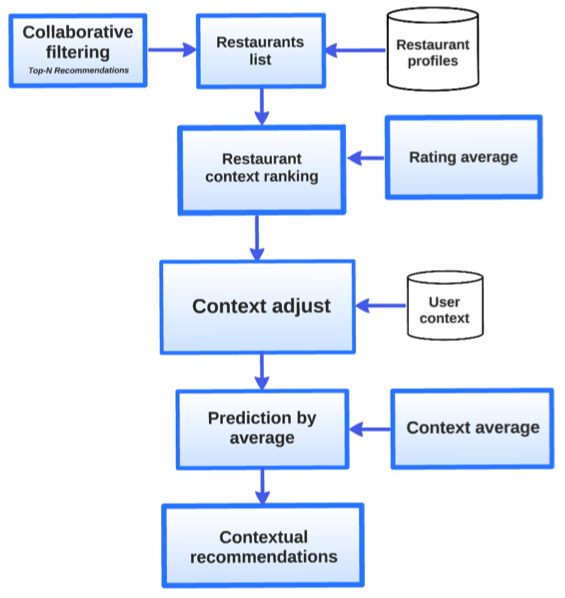
\includegraphics[width=0.60\textwidth]{img/posfil.png}}
	\caption{The Post-Filtering architecture for Tijuana restaurants.}
	\label{fig:postfiltering}     
\end{figure*}

This version includes 30 diffuse rules designed in an empiric way.
Two punctual differences exist in this version, the first one represented by the ranking value used in the users modeling based on graphs; the second one represents the usability elements adding a video game competitiveness paradigm.   Inside figure X we will appreciate the interface design added to EvoDrawing 03 version.

\begin{figure*}
	%\captionsetup{justification=centering,margin=2cm}
	\centering
	\setlength\fboxsep{0pt}
	\fbox{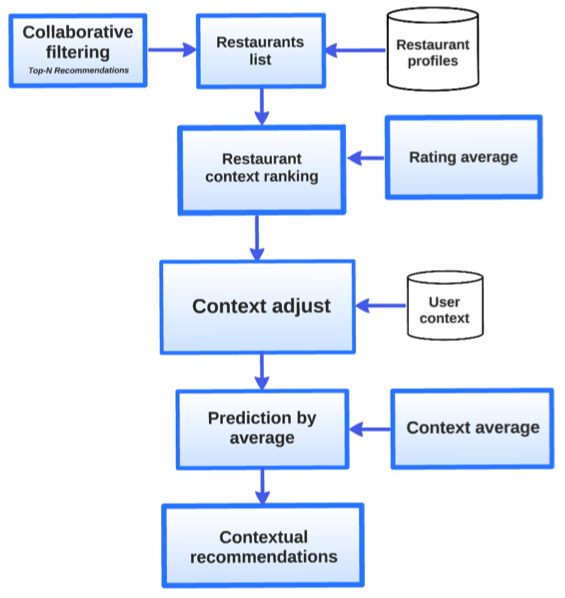
\includegraphics[width=0.60\textwidth]{img/posfil.png}}
	\caption{The Post-Filtering architecture for Tijuana restaurants.}
	\label{fig:postfiltering}     
\end{figure*}


Visual elements added to the navigation bar are added to this version, items such as the score where users can view its participations in EvoDrawings, it also provides you with the experience level acquired through their participation; This version will also offer an option to vie the leader chart inside the application as can we appreciate in figure x. The chart will show the ten best users and how many times they participate up to date.

\begin{figure*}
	%\captionsetup{justification=centering,margin=2cm}
	\centering
	\setlength\fboxsep{0pt}
	\fbox{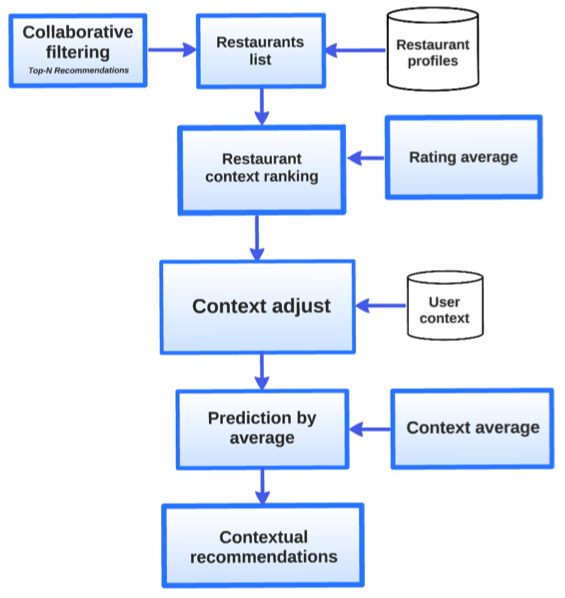
\includegraphics[width=0.60\textwidth]{img/posfil.png}}
	\caption{The Post-Filtering architecture for Tijuana restaurants.}
	\label{fig:postfiltering}     
\end{figure*}

Each experiment was promoted through social networking using specifically Facebook and  Twitter por medio de un URL corto asi como tambien un anuncio para motivar a los usuarios a presionar el link (URL corto). Esto con el fin encontrar participantes de forma voluntaria. Este URL corto se puede observar en la tabla x.

\begin{table}
	\small
	\caption{comparison of the different versions.}
	\label{tab:shorurl} 
	\centering
	\small
	\begin{tabular}{p{6cm} p{4cm}  }
		\hline\noalign{\smallskip}
		Long URL & Short URL  \\
		\noalign{\smallskip}\hline\noalign{\smallskip}
		\small{evodrawings01.herokuapp.com} & \small{goo.gl/J8TCe1}\\ \hline
		\small{evodrawings02.herokuapp.com} & \small{goo.gl/jqjNy5}\\ \hline
		\small{evodrawings03.herokuapp.com} & \small{goo.gl/J8TCe1}\\ \hline
		\noalign{\smallskip}\hline
	\end{tabular}
\end{table}

Is Worth to mention each experiment were implemented through a cloud service by using the  (Heroku) cloud service, in the following chart, each experiment will show its characteristics.

\begin{table}
	\small
	\caption{characteristics of  resources and services in cloud Heroku..}
	\label{tab:shorurl} 
	\centering
	\small
	\begin{tabular}{p{4cm} p{3cm} p{3cm} p{3cm}  }
		\hline\noalign{\smallskip}
		Service and resources & EvoDrawings01 & EvoDrawings02 & EvoDrawigs03 \\
		\noalign{\smallskip}\hline\noalign{\smallskip}
		\small{Heroku Free} & \small{\checkmark} & \small{\checkmark} & \small{\checkmark}\\ \hline
		\small{Deploy from Git} & \small{\checkmark} & \small{\checkmark} & \small{\checkmark}\\ \hline
		\small{Automated patching} & \small{\checkmark} & \small{\checkmark} & \small{\checkmark}\\ \hline
		\small{Self healing apps} & \small{\checkmark} & \small{\checkmark} & \small{\checkmark}\\ \hline
		\small{Undefined logs} & \small{\checkmark} & \small{\checkmark} & \small{\checkmark}\\ \hline
		\small{Number of process types} & \small{2} & \small{2} & \small{2}\\ \hline
		\small{Always on Sleep after 30 mins of inactivity, otherwise always on depending on you remaining mostly free dynes hours} & \small{\checkmark} & \small{\checkmark} & \small{\checkmark}\\ \hline
		\small{Custom domains} & \small{\checkmark} & \small{\checkmark} & \small{\checkmark}\\ \hline
		\small{RAM 512} & \small{\checkmark} & \small{\checkmark} & \small{\checkmark}\\ \hline
		\small{Dedicated} & \small{x} & \small{x} & \small{x}\\ \hline
		\small{Heroku Postgres ::DB Hobby Dev} & \small{\checkmark} & \small{\checkmark} & \small{\checkmark}\\ \hline
		\small{GrapheneDB Chalk} & \small{\checkmark} & \small{x} & \small{\checkmark}\\ \hline
		\small{Redis To Go Nano} & \small{\checkmark} & \small{x} & \small{\checkmark}\\ \hline
		\small{GrapheneDB Sandstone} & \small{x} & \small{x} & \small{\checkmark}\\ \hline
		\small{Redis To Go Mini} & \small{x} & \small{x} & \small{\checkmark}\\ \hline
		
		
		\noalign{\smallskip}\hline
	\end{tabular}
\end{table}

The experiments initial purpose is to design specific applications and interfaces to achieve user participation in a voluntary way in every single application. Each experiment allowed the commitment to obtain data to be used later  to evaluate and analyze which version had the most user participation; To prove the initial hypothesis we implemented 3 study cases with slight differences in its configuration characteristics to each application allowing us enabling us to decide through obtained results which of the study cases prove this investigation hypothesis. Next chapter will show the Obtained results in the survey.


